@@ -1,465 +0,0 @@
\section{Tables}\label{Appendix:Tables}
\subsubsection{Gregor -- Keyboard Shorcuts}
{
\begin{table}[ht]
    \centering
    \resizebox{\textwidth}{!}{\begin{tabular}{| p{0.35\linewidth} | p{0.6\linewidth} |}
      \hline
      % after \\: \hline or \cline{col1-col2} \cline{col3-col4} ...
      Key & Action \\
      \hline
      \multicolumn{2}{|c|}{The File Menu} \\
      \hline
      Ctrl + O & Open an existing document \\
      Ctrl + S & Save the document to the last selected file or a new file if no previous file is associated. \\
      Ctrl + Shift + S & Save the data in a new file \\
      Ctrl + I & Import spline data from file \\
      Ctrl + E & Open up the export menu \\
      Shift + Del  & Clear the workspace \\
      Alt + F4 & Close the application \\
      \hline
      \multicolumn{2}{|c|}{The View Menu} \\
      \hline
      Ctrl + 4 & Combined Mode; Shows both ink and curves \\
      Ctrl + 5 & Ink Only Mode; Shows Only the ink marks and hides the curve alogwith the handles \\
      Ctrl + 6 & Splines Mode. Hides the ink marks \\
      Ctrl + G & Toggle the visibility of the grid \\
      Ctrl + Shift B & Toggle the visibility of the background images \\
      \hline
      \multicolumn{2}{|c|}{The Edit Menu} \\
      \hline
      Ctrl + 1 & Toggles the splines anchor centers \\
      Ctrl + 2 & Toggles the splines curvature handles \\
      Ctrl + 3 & Toggles the rotation handles \\
      Ctrl + V & Toggles the action of mouse left click between adding the anchor and dragging the workspace. \\
      \hline
      \multicolumn{2}{|c|}{Help}\\
      \hline
      F1 & Shows quick help \\
      F2 & Opens up the project Git.\\
      \hline
    \end{tabular}}
    \label{Table:Keyboardshortcuts}
    \end{table}
}
\clearpage
\section{Source Code}\label{Appendix:sourceCode}
{
    \clearpage
}
\section{Code Snippets}\label{Appendix:CodeSnippets}
{
\begin{lstlisting}[language=XML]
//Sample code of a rotating Bezier spline that will render the Urdu letter Aa'en in Nastaleeq.
<spline>
    <FlatTipWidth>150</FlatTipWidth>
    <Color>-5658199</Color>
    <anchor>
      <rotationoffset>0</rotationoffset>
      <P>-198.3791, 452.6993</P>
      <C1>-131.6351, 572.4461</C1>
      <C2>-265.1234, 332.9534</C2>
      <R1>-148.3791, 452.6993</R1>
    </anchor>
    <anchor>
      <rotationoffset>0</rotationoffset>
      <P>-296.5323, 156.2775</P>
      <C1>-439.8357, 254.4304</C1>
      <C2>-119.5302, 35.04326</C2>
      <R1>-246.5322, 156.2775</R1>
    </anchor>
    <anchor>
      <rotationoffset>0</rotationoffset>
      <P>25.40986, 374.1774</P>
      <C1>-47.22344, 262.2825</C1>
      <C2>98.04301, 486.0714</C2>
      <R1>75.40986, 374.1774</R1>
    </anchor>
    <anchor>
      <rotationoffset>0</rotationoffset>
      <P>-233.7143, -183.332</P>
      <C1>-208.1945, -28.25013</C1>
      <C2>-274.7982, -432.9961</C2>
      <R1>-183.7143, -183.332</R1>
    </anchor>
    <anchor>
      <rotationoffset>0</rotationoffset>
      <P>315.9428, -517.0526</P>
      <C1>95.77186, -679.5702</C1>
      <C2>435.6645, -428.6809</C2>
      <R1>365.9427, -517.0526</R1>
    </anchor>
    <anchor>
      <rotationoffset>0</rotationoffset>
      <P>441.5787, -144.0708</P>
      <C1>388.576, -277.5591</C1>
      <C2>494.5813, -10.58265</C2>
      <R1>491.5787, -144.0708</R1>
    </anchor>
  </spline>
\end{lstlisting}
}
\section{Images}
{

\begin{figure}[H]
  \centering
  \includegraphics[width=0.8\textwidth]{../Images/Nastaleeq_Ink.pdf}
  \caption
  {
      Nastaleeq sample by Gohar Qalam. (a) Original calligraphy photo. (b) Original photo processed for analysis. (c) Traced rotating bezier spline ink. (d) Difference between (b) and (c). The red pixel indicate the portions that are missing in (c) but are present in (b) and the blue ones show the missing pixels in (b) but are present in (c).
  }
\end{figure}

\begin{figure}[H]
  \centering
  
\includegraphics[width=0.8\textwidth]{../Images/Nastaleeq_Machined.pdf}
  \caption
  {
      Machined Nastaleeq sample by Gohar Qalam. (a) Rasterized rotating bezier spline for machining (b) Ink marks machined by a simulated robotic manipulator. (c) and (d) are differences between simulated ink mark and the rasterized photo and the processed original photo respectively. The red pixel indicate the portions that are missing in (c) but are present in the reference image and the blue ones show the missing pixels in reference but are present in the ink mark.
  }
\end{figure}

\begin{figure}[H]
  \centering
  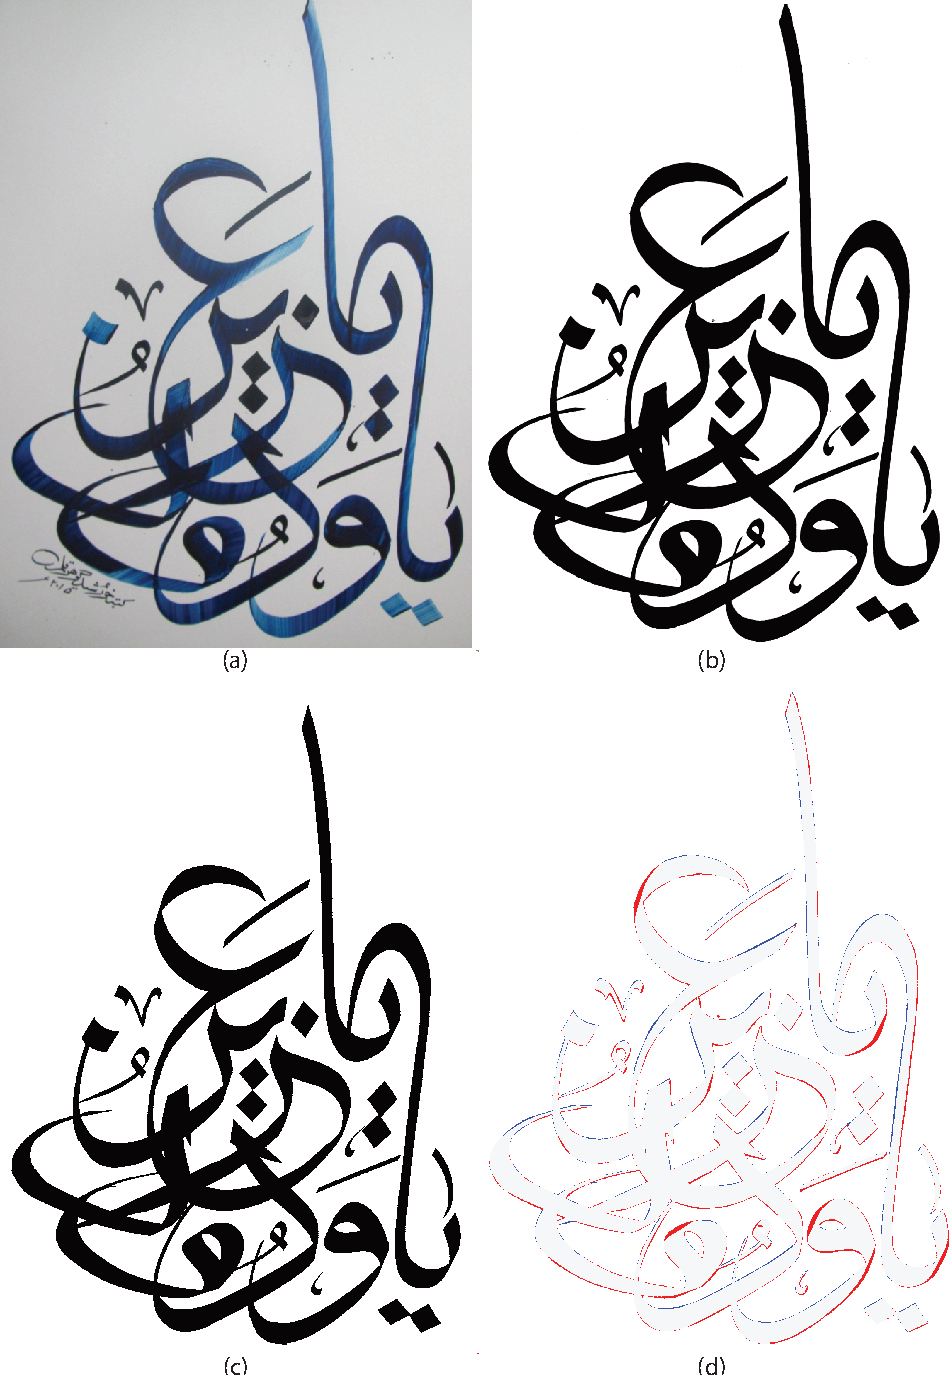
\includegraphics[width=0.8\textwidth]{../Images/Thuluth_Ink.pdf}
  \caption
  {
      Thuluth sample by Gohar Qalam. (a) Original calligraphy photo. (b) Original photo processed for analysis. (c) Traced rotating bezier spline ink. (d) Difference between (b) and (c). The red pixel indicate the portions that are missing in (c) but are present in (b) and the blue ones show the missing pixels in (b) but are present in (c).
  }
\end{figure}

\begin{figure}[H]
  \centering
  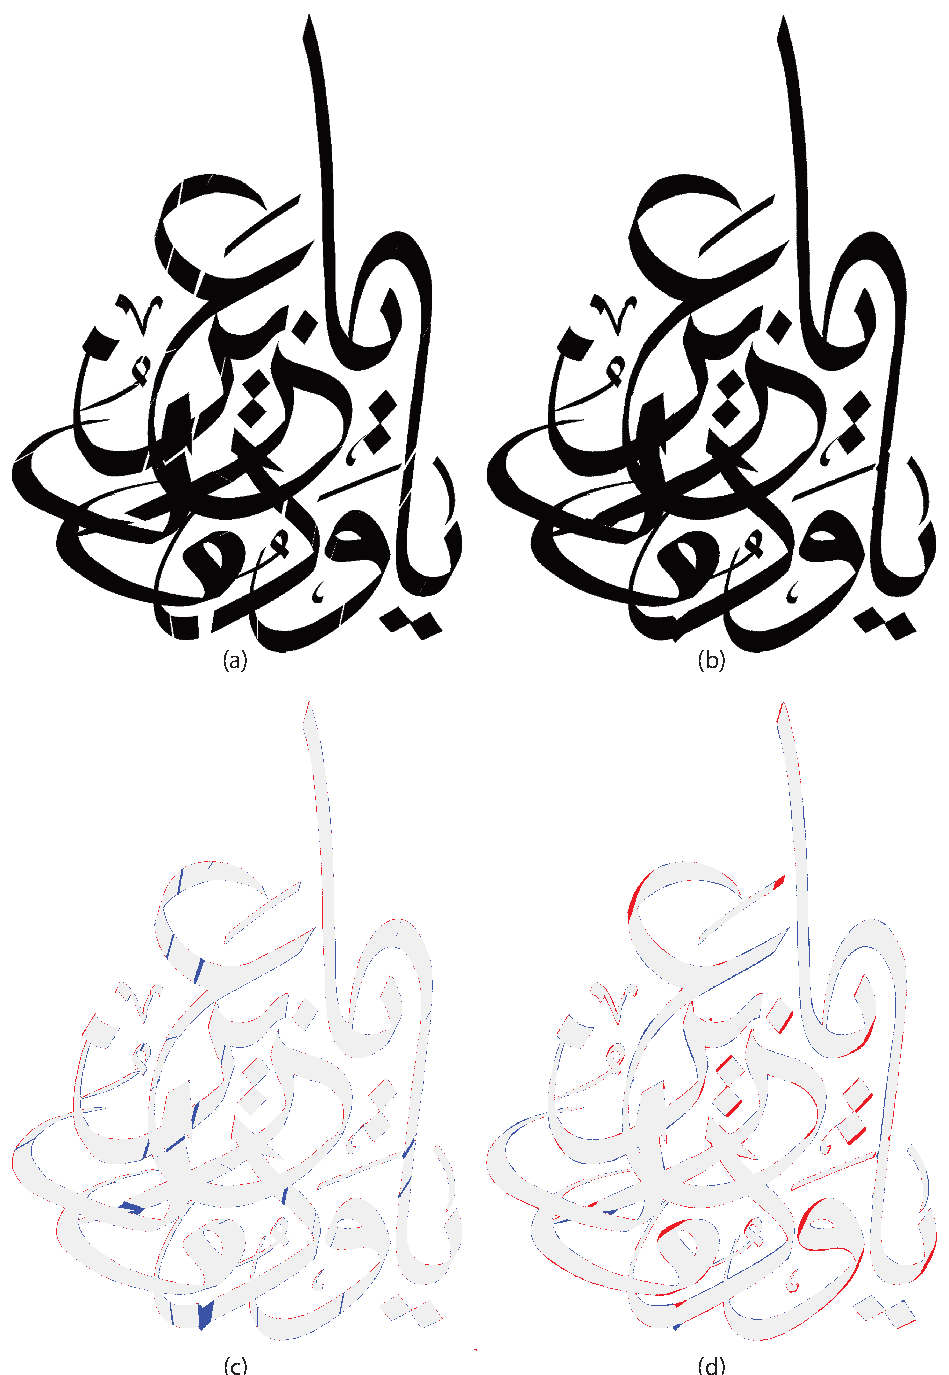
\includegraphics[width=0.8\textwidth]{../Images/Thuluth_Machined.pdf}
  \caption
  {
      Machined Thuluth sample by Gohar Qalam. (a) Rasterized rotating bezier spline for machining (b) Ink marks machined by a simulated robotic manipulator. (c) and (d) are differences between simulated ink mark and the rasterized photo and the processed original photo respectively. The red pixel indicate the portions that are missing in (c) but are present in the reference image and the blue ones show the missing pixels in reference but are present in the ink mark.
  }
\end{figure}
}